\documentclass{sbc2023}%

\usepackage{graphicx}
%\usepackage[utf8]{inputenc}
\usepackage[misc,geometry]{ifsym} 
\usepackage{fontspec}
\usepackage{fontawesome}
\usepackage{academicons}
\usepackage{color}
\usepackage{hyperref} 
\usepackage{aas_macros}
\usepackage[bottom]{footmisc}
\usepackage{supertabular}
\usepackage{afterpage}
\usepackage{url}
\usepackage{pifont}
\usepackage{multicol}
\usepackage{multirow}

\setcitestyle{square}

\definecolor{orcidlogo}{rgb}{0.37,0.48,0.13}
\definecolor{unilogo}{rgb}{0.16, 0.26, 0.58}
\definecolor{maillogo}{rgb}{0.58, 0.16, 0.26}
\definecolor{darkblue}{rgb}{0.0,0.0,0.0}
\hypersetup{colorlinks,breaklinks,
            linkcolor=darkblue,urlcolor=darkblue,
            anchorcolor=darkblue,citecolor=darkblue}
%\hypersetup{colorlinks,citecolor=blue,linkcolor=blue,urlcolor=blue}

%%%%%%% IMPORTANT: We disable hyperlinks by default with this line, to avoid the error "\pdfendlink ended up in different nesting level" while writing.
%\hypersetup{draft}

\jid{JBCS}
\jtitle{Journal of the Brazilian Computer Society, 202X, XX:1, }
\doi{10.5753/jbcs.202X.XXXXXX}
\copyrightstatement{This work is licensed under a Creative Commons Attribution 4.0 International License}
\jyear{202X}


\title[Metodos de Identificação de Arestas de Ponte]{Metodos de Identificação de Arestas de Ponte}

%THE ORCID IS MANDATORY FOR EACH AUTHOR IN JBCS
\author[Viterbo et al. 202X]{
\affil{\textbf{Vitor Oliveira}~\href{https://orcid.org/0000-0002-7110-2026}{\textcolor{orcidlogo}{\aiOrcid}}~~[~\textbf{ Pontifical Catholic University of Minas Gerais}~|\href{mailto:vitor.lucio.0916@gmail.com}{~\textbf{\textit{vitor.lucio.0916@gmail.com}}}~]}

\affil{\textbf{João Vítor Scarlatelli}~\href{https://orcid.org/0000-0002-7110-2026}{\textcolor{orcidlogo}{\aiOrcid}}~~[~\textbf{ Pontifical Catholic University of Minas Gerais}~|\href{mailto:jvitorfreitas2004@gmail.com}{~\textbf{\textit{jvitorfreitas2004@gmail.com}}}~]}

\affil{\textbf{Ana Maria Rafael}~\href{https://orcid.org/0000-0003-3052-3016}{\textcolor{orcidlogo}{\aiOrcid}}~~[~\textbf{ Pontifical Catholic University of Minas Gerais}~|\href{mailto:amrrafael@sga.pucminas.br}{~\textbf{\textit{amrrafael@sga.pucminas.br}}}~]}

\affil{\textbf{Nagib Borjaili}~\href{https://orcid.org/0000-0002-2431-8457}{\textcolor{orcidlogo}{\aiOrcid}}~~[~\textbf{ Pontifical Catholic University of Minas Gerais~}|\href{mailto:nagibverly@gmail.com}{~\textbf{\textit{nagibverly@gmail.com}}}~]}

\affil{\textbf{Yasmin Viegas}~\href{https://orcid.org/0000-0002-2431-8457}{\textcolor{orcidlogo}{\aiOrcid}}~~[~\textbf{ Pontifical Catholic University of Minas Gerais~}|\href{mailto:yasminviegas98@gmail.com}{~\textbf{\textit{yasminviegas98@gmail.com}}}~]}


}

\begin{document}

\begin{frontmatter}
\maketitle



\begin{abstract}
\textbf{Abstract.~}
\noindent A identificação de pontes em grafos é um problema fundamental na teoria dos grafos, com aplicações em redes computacionais, otimização de rotas e análise de vulnerabilidades estruturais. Este relatório compara dois métodos para detectar essas arestas críticas: o método \textit{Naive}, baseado na remoção e verificação da conectividade, e o método de \textit{Tarjan}, que utiliza busca em profundidade (DFS) para identificar pontes de forma eficiente. A análise de complexidade mostra que o método \textit{Naive} tem custo $O(V^4)$ em grafos densos, tornando-se inviável para grandes escalas, enquanto o método de \textit{Tarjan} opera em $O(V^2)$, sendo significativamente mais eficiente. Os resultados reforçam a importância da escolha de algoritmos otimizados para aplicações em grafos densos. 
\end{abstract}

\begin{keywords}
Grafos, Pontes, Vértices, Arestas, Conectividade, Complexidade 
\end{keywords}

%\begin{license}
%Published under the Creative Commons Attribution 4.0 International Public License (CC BY 4.0)
%\end{license}

\end{frontmatter}


\section{Introdução}
\label{sec:intro}

O problema de determinar pontes em um grafo (também conhecidas como arestas de corte) é um dos desafios fundamentais na teoria dos grafos, tendo aplicações práticas em diversas áreas, como análise de redes, otimização de rotas e segurança de sistemas. Pontes são arestas críticas que, quando removidas, aumentam o número de componentes conexos do grafo, desconectando-o. Esse conceito é usado, por exemplo, para identificar vulnerabilidades em redes de computadores, projetar circuitos elétricos robustos ou até mesmo analisar redes sociais e ecológicas.

Além disso, a identificação de pontes está diretamente relacionada a problemas clássicos da teoria dos grafos, como a determinação de caminhos ou ciclos eulerianos. A eficiência na detecção dessas arestas auxilia na otimização do desempenho de algoritmos projetados para processar ou analisar grafos de grande escala.

Este relatório explora técnicas para a identificação de pontes em grafos, comparando dois métodos principais: o método \textbf{Naive} (ingênuo), que verifica a conectividade do grafo após a remoção de cada aresta, e o método baseado em  \textbf{\cite{ref5}}, que utiliza uma abordagem baseada em DFS (Busca em Profundidade), para identificar pontes diretamente. Além disso, o estudo avalia o desempenho desses métodos quando integrados ao algoritmo de \cite{ref6}, analisando sua eficiência e aplicabilidade na resolução de problemas relacionados à identificação de ciclos eulerianos em grafos.

Ao analisar esses métodos, este trabalho busca não apenas apresentar suas implementações, mas também discutir seu custo/complexidade, contribuindo para uma compreensão mais aprofundada desses métodos e do problema.

\section{Metodologia}
Para implementar os métodos baseados em \textbf{Naive} e \textbf{Tarjan}, no algortimo de Fleury, a estrutura de \textbf{lista de adjacência} foi utilizada em ambos os casos para representar os grafos. Uma lista de adjacência é uma coleção de listas ou vetores, em que cada vértice do grafo possui uma lista indicando os vértices aos quais está conectado por uma aresta.


Exemplo: \textit{G = (V, E)}, \( V= \{A, B, C, D\} \) e arestas \( E = \{(A, B), (A, C), (B, D), (C, D)\} \). A representação desse grafo em lista de adjacência é dada pela tabela abaixo:

\begin{center}
\begin{tabular}{|c|c|}
\hline
\textbf{Vértice} & \textbf{Lista de Adjacência (Vizinhos)} \\
\hline
A & B, C \\
\hline
B & A, D \\
\hline
C & A, D \\
\hline
D & B, C \\
\hline
\end{tabular}
\end{center}

Além da lista de adjacência, cada implementação possui métodos exclusivos para a identificação de pontes. A única funcionalidade comum entre ambas é o método de adição de arestas ao grafo, que garante a consistência da estrutura de dados durante a execução dos algoritmos.

\subsection{Método Naive}
Considerando um grafo não direcionado \textit{G = (V, E)}, o método Naive segue uma abordagem de força bruta para identificar arestas de ponte. Sua implementação foi dividida em quatro etapas principais:
\begin{itemize}
\item \textbf{Listar todas as arestas}: Percorre a lista de adjacência para armazenar cada aresta única em um vetor, evitando duplicações em grafos não direcionados.
\item \textbf{Remover aresta}: Remove temporariamente uma aresta \textit{E} do grafo \textit{G}.
\item \textbf{Testar conectividade}: Realiza uma busca em largura (BFS) para verificar se o grafo permanece conexo após a remoção da aresta.
\item \textbf{Adicionar aresta}: Reinsere a aresta no grafo para continuar a iteração com as arestas subsequentes.
\end{itemize}

O processo é repetido para cada aresta \textit{E} do grafo \textit{G}, exceto pela etapa de listagem, que é realizada apenas uma vez. Se o grafo deixar de ser conexo após a remoção de uma aresta, essa aresta é classificada como uma ponte.

\subsubsection{Análise do Custo Computacional}
Para analisar o custo do algoritmo, é necessário detalhar os métodos auxiliares utilizados:
\begin{itemize}
\item \textbf{Adicionar Arestas}: Adiciona uma aresta à lista de adjacência. \textit{O(1)}.
\item \textbf{Remover Arestas}: Remove uma aresta da lista de adjacência.  \textit{O(V)} no pior caso.
\item \textbf{Teste de Conectividade}: Verifica a conectividade do grafo usando BFS. No pior caso (quando \textit{G} é conexo), todos os vértices \textit{V} e arestas \textit{E} são percorridos.  \textit{O(V + E)}.
\item \textbf{Identificar Pontes}: Executa o teste de conectividade para cada aresta.  \textit{O(E * (V + E))}.
\end{itemize}



O custo total do algoritmo Naive é dominado pela \textbf{identificação de pontes}, uma vez que todos os métodos auxiliares são executados dentro dela. O principal fator de custo é a busca em largura (BFS), que é realizada a cada remoção de aresta para verificar a conectividade do grafo. Como a BFS tem complexidade \textit{O(V + E)} e é executada \textit{E} vezes (uma vez para cada aresta), o custo total do algoritmo é \textit{O(E * (V + E))}.

Além disso, a complexidade de \textbf{adicionar arestas} e \textbf{remover aresta} não são relevantes no cálculo do custo total, pois esses métodos têm custos muito menores em comparação com o custo dominante da BFS. Enquanto \textbf{adicionar arestas} tem complexidade\textit{ O(1)} e \textbf{remover arestas} tem complexidade \textit{O(V)} no pior caso, o custo de \textbf{identificar pontes} \textit{O(E * (V + E))} domina completamente a complexidade total do algoritmo.

\subsection{Método de Tarjan}
Considerando um grafo não direcionado \textit{G = (V, E)}, o método de Tarjan utiliza uma abordagem baseada em \textbf{Busca em Profundidade} (DFS, Depth-First Search) para identificar arestas de ponte de forma eficiente. Diferentemente do método Naive, que verifica a conectividade do grafo após a remoção de cada aresta, o método de Tarjan identifica pontes em uma única passagem de DFS, aproveitando os conceitos de \textbf{tempo de descoberta} e \textbf{\textit{low value}} (valor mínimo) para cada vértice.

O tempo de descoberta refere-se ao momento em que o vértice é visitado durante a busca em profundidade, iniciando-se em 0 para o primeiro vértice. Já o \textit{low value} representa o ancestral mais antigo, excluindo o vértice pelo qual foi acessado (no caso de uma representação em árvore, seria o nó pai), associado ao vértice em visita. Esses conceitos permitem ao algoritmo determinar de forma eficiente se uma aresta é uma ponte, comparando os valores de tempo de descoberta e \textit{low value} durante a execução da DFS.

A implementação do método de Tarjan foi dividida nas seguintes etapas principais:
\begin{itemize}
\item \textbf{Inicialização}: Para cada vértice do grafo, são inicializados os valores de tempo de descoberta, \textit{low value} e um vetor de visitados.
\item \textbf{DFS}: Durante a DFS, o algoritmo calcula o \textit{low value} de cada vértice, que representa o menor tempo de descoberta alcançável a partir desse vértice. Se o \textit{low value} de um vértice vizinho for maior que o tempo de descoberta do vértice atual, a aresta entre eles é classificada como uma ponte.
\end{itemize}

O método de Tarjan é executado em uma única passagem de DFS, o que resulta em uma complexidade computacional significativamente menor em comparação ao método Naive.

\subsubsection{Análise do Custo Computacional}
Para analisar o custo do algoritmo de Tarjan, é necessário detalhar os principais componentes:
\begin{itemize}
\item \textbf{DFS}: A busca em profundidade é realizada uma vez para cada componente conexo do grafo. No pior caso, todos os vértices (V) e arestas (E) são visitados. Complexidade: \textit{O(V + E)}.
\item \textbf{Cálculo do \textit{low value}}: Durante a DFS, o \textit{low value} é calculado para cada vértice V, o que não adiciona custo adicional significativo, pois é feito em conjunto com a DFS.
\item \textbf{Identificação de pontes}: A verificação de pontes é realizada em tempo constante \textit{O(1)} para cada aresta durante a DFS.
\end{itemize}

O custo total do algoritmo de Tarjan é dominado pela DFS, resultando em uma complexidade de\textit{ O(V + E)}. Isso ocorre porque o algoritmo visita cada vértice e aresta uma única vez, sem a necessidade de repetir operações custosas, como no método Naive.

\subsection{Visualização dos métodos}

Utilizando o grafo \textit{G=(V,E)}, não direcionado, ilustrado na figura abaixo, podemos exemplificar o funcionamento da detecção de pontes pelos métodos Naive e Tarjan. Neste caso, a aresta \textit{(f, g)} é a única ponte presente no grafo: 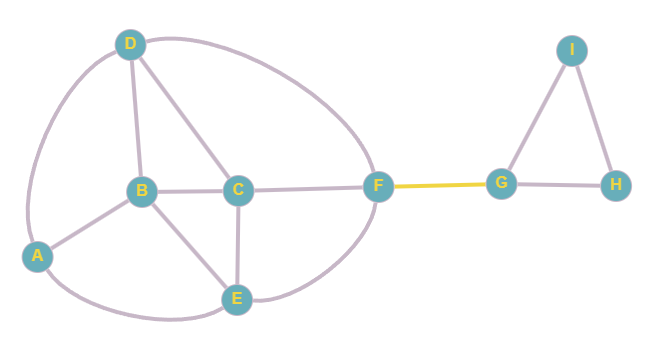
\includegraphics[width=\columnwidth]{grafo.png}

\subsubsection{Naive}
No método Naive, podemos observar que, em algum momento durante sua execução, a aresta \textit{(f, g)} é removida do grafo. A partir disso, é realizada uma análise de conectividade em todo o grafo. Neste caso, como o número de componentes conexos aumenta, a aresta é identificada como uma ponte. 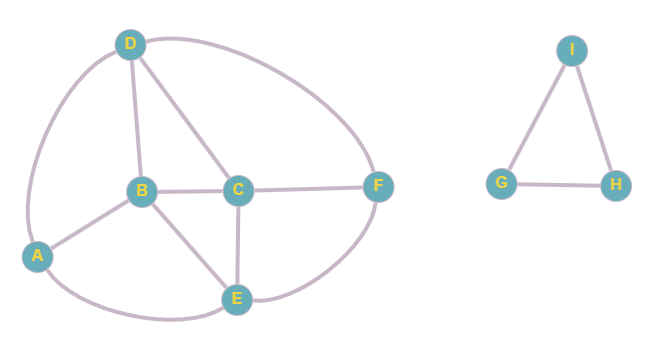
\includegraphics[width=\columnwidth]{grafo_naive.png}

\subsubsection{Tarjan}
No método Tarjan, podemos observar que é realizada uma busca em profundidade, marcando os tempos de descoberta (em azul) e os \textit{low values} (em vermelho). Durante a execução da busca, a aresta \textit{(f, g)} é identificada como ponte, uma vez que o \textit{low value} do vértice \textit{g} é maior que o tempo de descoberta do vértice \textit{f}.
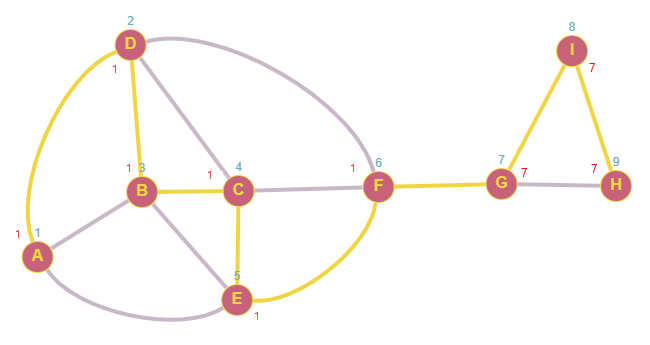
\includegraphics[width=\columnwidth]{grafo_tarjan-2.png}




\section{Analise de custo e resultados}

Nesta seção, avaliamos o impacto do custo computacional dos métodos \textit{Naive} e \textit{Tarjan} em grafos densos. Grafos densos são aqueles em que o número de arestas $E$ é proporcional ao quadrado do número de vértices $V$, ou seja, 
$ E \approx V^2. $
Essa característica é comum em grafos completos ou em grafos com alta conectividade, onde a maioria dos vértices está interconectada.


\begin{itemize}
    \item\textbf{Método Naive:} \( O(E \cdot (V + E)) \). Para grafos densos, \( E \approx V^2 \), então a complexidade se torna: \[O(V^2 \cdot (V + V^2)) = O(V^4).\]

    \item\textbf{Método de Tarjan:} \( O(V + E) \). Para grafos densos, \( E \approx V^2 \), então a complexidade se torna:\[O(V + V^2) = O(V^2).\]
\end{itemize}

Considerando os caculos, na tabela a seguir é apresentado uma comparação dos tempos teóricos estimados para os métodos em grafos de diferentes tamanhos. Para os cálculos, foi considerada uma complexidade temporal em que cada operação básica leva 1 nanossegundo (ns). Os tempos foram calculados para grafos com \( V = 100 \), \( V = 1.000 \), \( V = 10.000 \) e \( V = 100.000 \) vértices, assumindo que o número de arestas \( E \) é proporcional a \( V^2 \) (grafos densos).


\begin{table}[h]
    \centering
    \label{tab:comparacao}
    \small % Reduz o tamanho da fonte da tabela
    \renewcommand{\arraystretch}{1.2} % Aumenta um pouco o espaçamento vertical
    \setlength{\tabcolsep}{5pt} % Reduz o espaçamento entre colunas
    \resizebox{\linewidth}{!}{ % Ajusta a tabela para caber na largura da página
    \begin{tabular}{|c|c|c|c|}
        \hline
        \textbf{Número de Vértices (\(V\))}  & \textbf{Método Naive (\(O(V^4)\))} & \textbf{Método de Tarjan (\(O(V^2)\))} \\
        \hline
        100  & \(100\) ms & \(0,01\) ms \\
        \hline
        1.000   & \(16,67\) minutos & \(1\) ms \\
        \hline
        10.000  & \(115,74\) dias & \(100\) ms \\
        \hline
        100.000  & \(3,17\) milhões de anos & \(10\) segundos \\
        \hline
    \end{tabular}
    }
     \caption{Tempos teóricos de Naive e Tarjan.}
\end{table}

Como esperado, o método Naive, com complexidade \(O(V^4)\), cresce rapidamente e se torna inviável para grafos grandes, chegando a tempos astronômicos para \(V = 100.000\). Por outro lado, o método de Tarjan, com complexidade \(O(V^2)\), apresenta um crescimento significativamente mais lento, permanecendo computacionalmente viável mesmo para valores altos de \(V\). Essa diferença evidencia a importância de algoritmos mais eficientes para o processamento de grafos densos.



\section{Conclusão}
Este relatório explorou dois métodos para a identificação de arestas de ponte em grafos: o método Naive e o método proposto por \cite{ref5}. Por meio da implementação e análise dessas abordagens, foi possível demonstrar a eficácia e a eficiência na identificação de pontes, utilizando o algoritmo apresentado por \cite{ref6}.

O método Naive possui uma implementação mais simples e direta, o que facilita sua visualização e interpretação. No entanto, essa simplicidade tem um custo em termos de desempenho, uma vez que sua lógica básica resulta em uma grande repetição de operações. Consequentemente, sua ordem de complexidade chega a \(O(V^4)\) em grafos mais densos, o que o torna menos eficiente.

Por outro lado, o método de Tarjan, embora apresente uma implementação mais complexa, oferece uma eficiência significativamente superior à do método Naive. Isso ocorre porque suas operações são otimizadas, exigindo apenas uma única passagem por todo o grafo. Essa característica reduz drasticamente o custo computacional, resultando em uma complexidade muito mais favorável, 
\(O(V^2)\), em grafos densos. No entanto, a correção do método de Tarjan, quando integrado ao algoritmo de Fleury, não é estável. Isso se deve ao fato de que, durante a execução do algoritmo de Fleury, ocorre a remoção de arestas, e, com isso, outras arestas podem se tornar pontes. Consequentemente, as pontes previamente identificadas pelo Tarjan podem não ser suficientes para garantir a corretude do caminho euleriano formado. A única forma de garantir essa corretude seria executar o método de Tarjan novamente a cada remoção de aresta, o que, na prática, o tornaria equivalente ao método Naive, tanto em custo computacional quanto em raciocínio.

Em síntese, a escolha entre o método Naive e o método de Tarjan depende do contexto de aplicação e dos requisitos de desempenho. Enquanto o método Naive se destaca por sua simplicidade e precisão, o método de Tarjan oferece uma solução mais robusta e eficiente para grafos de maior densidade. No entanto, é importante ressaltar que, ao integrar o método de Tarjan ao algoritmo de Fleury, sua corretude pode ser comprometida devido à dinâmica de remoção de arestas, que pode transformar outras arestas em pontes durante a execução. Portanto, para cenários que demandam alta performance e não envolvem a remoção dinâmica de arestas, o método de Tarjan é claramente a abordagem mais vantajosa. Esta análise reforça a importância de se considerar tanto a clareza quanto a eficiência e a estabilidade na seleção de algoritmos para problemas complexos, como a identificação de arestas de ponte em grafos

\section{Divisão de Tarefas}
\begin{itemize}
\item \textbf{Vitor Lúcio:} Documentação e formatação do trabalho;
\item \textbf{Nagib Borjaili:} Implementação do método Naive;
\item \textbf{João Vítor Scarlatelli e Yasmin Viegas:} Implementação do método Tarjan;
\item \textbf{Ana Maria Rafael:} Implementação do algoritmo de Fleury utilizando os métodos Tarjan e Naive.
\end{itemize}

\bibliographystyle{plainnat}
\bibliography{refs}

\end{document}
